\documentclass[border=5pt]{standalone}
\usepackage{tikz}
\usepackage{amsmath}
\begin{document}
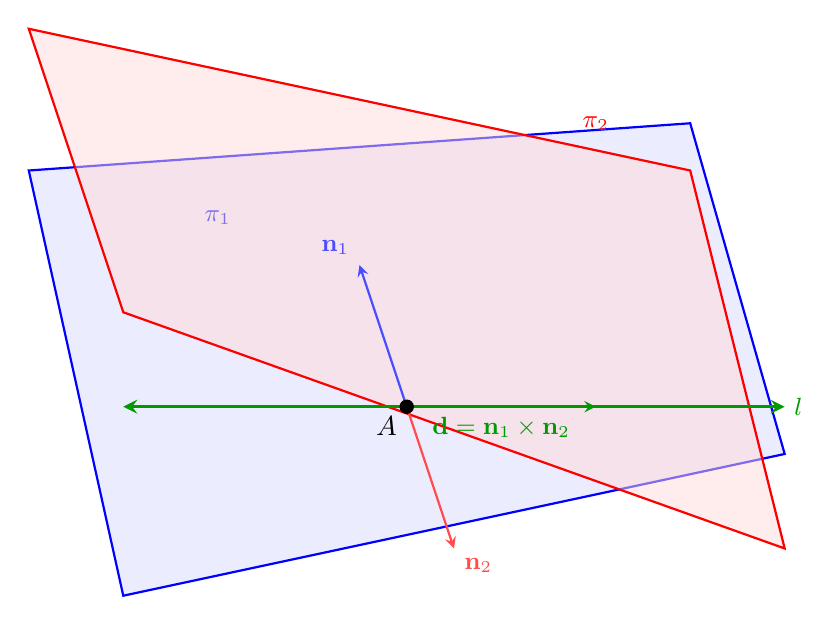
\begin{tikzpicture}[scale=1.2, >=stealth]
  % Two planes intersecting in a line

  % Plane 1 (light blue)
  \fill[blue!15, opacity=0.5] (-3, -1) -- (4, 0.5) -- (3, 4) -- (-4, 3.5) -- cycle;
  \draw[thick, blue] (-3, -1) -- (4, 0.5) -- (3, 4) -- (-4, 3.5) -- cycle;
  \node[blue, font=\small] at (-2, 3) {$\pi_1$};

  % Plane 2 (light red)
  \fill[red!15, opacity=0.5] (-3, 2) -- (4, -0.5) -- (3, 3.5) -- (-4, 5) -- cycle;
  \draw[thick, red] (-3, 2) -- (4, -0.5) -- (3, 3.5) -- (-4, 5) -- cycle;
  \node[red, font=\small] at (2, 4) {$\pi_2$};

  % Intersection line
  \draw[very thick, green!60!black, <->] (-3, 1.0) -- (4, 1.0);
  \node[green!60!black, font=\small, right] at (4, 1.0) {$l$};

  % Direction vector of line
  \draw[->, thick, green!60!black] (0, 1.0) -- (2, 1.0) node[midway, below, font=\small] {$\mathbf{d} = \mathbf{n}_1\times\mathbf{n}_2$};

  % Normal vectors
  \draw[->, thick, blue!70] (0, 1.0) -- (-0.5, 2.5) node[above left, font=\small] {$\mathbf{n}_1$};
  \draw[->, thick, red!70] (0, 1.0) -- (0.5, -0.5) node[below right, font=\small] {$\mathbf{n}_2$};

  % Point on intersection
  \filldraw[black] (0, 1.0) circle (2pt) node[below left] {$A$};
\end{tikzpicture}
\end{document}
